\chapter{Numerical Calculations}

Numerical transport calculations have a huge advantage over the analytical
calculation: once a formalism is implemented, it works for arbitrary
configurations within the limits of the model. However, it does not generally
supply us with data that enhances physical understanding, so it is best use as a
means to expand on analytical calculations which we already understand.

In that spirit we performed numeric calculations, simulating a sample with
Rashba Spin-orbit coupling, and spin-resolved leads attached at the edges.

The calculation follows this rough scheme:

\begin{itemize}
    \item set up the Hamiltonian $H$
    \item calculate the self-energy matrices $\Sigma_p$
    \item calculate the Green's functions $G^A$ and $G^R$ by inverting
          $H + \sum_p \Sigma_p$
    \item use the Fisher-Lee relation to calculate the transmission matrix $T$
            from $G^R$, $G^A$ and $\Sigma_p$
\end{itemize}

\section{Performance Consideration}

These numeric calculations are computationally expensive. If we simulate a
lattice with a total of $n \times n$ sites, the matrices $H$, $\Sigma_p$, $G^R$ and
$G^A$ are of dimensions $2n^2 \times 2n^2$. Inversion of an $m \times m $
matrix and multiplication of two $ m \times m $ matrices, both take $O(m^3)$
steps\footnote{There are matrix product algorithms with slightly better
asymptotic scaling, but they are usually very complicated, numerically badly
conditioned or only advantageous for huge systems; usually all three apply}
\cite{matrixperformance}. All other steps are faster and can be ignored for
an asymptotic analysis.

So the naive approach takes $O(n^6)$ steps for $n \times n$ lattice sites.

An alternative approach, the \emph{Recursive Green's Function method} works by
decomposing the sample into slices in such a way that the sites in each slice
only interact with neighbor slices. For short range interactions such a
decomposition can be found, and for nearest-neighbor hopping the time
complexity approaches $O(n^3)$ \cite{rgfschmelcher}. However, this is payed by
a significantly increased implementation complexity, and the algorithm is tied
to the specific form of the Hamiltonian.

\begin{figure}
    \begin{center}
    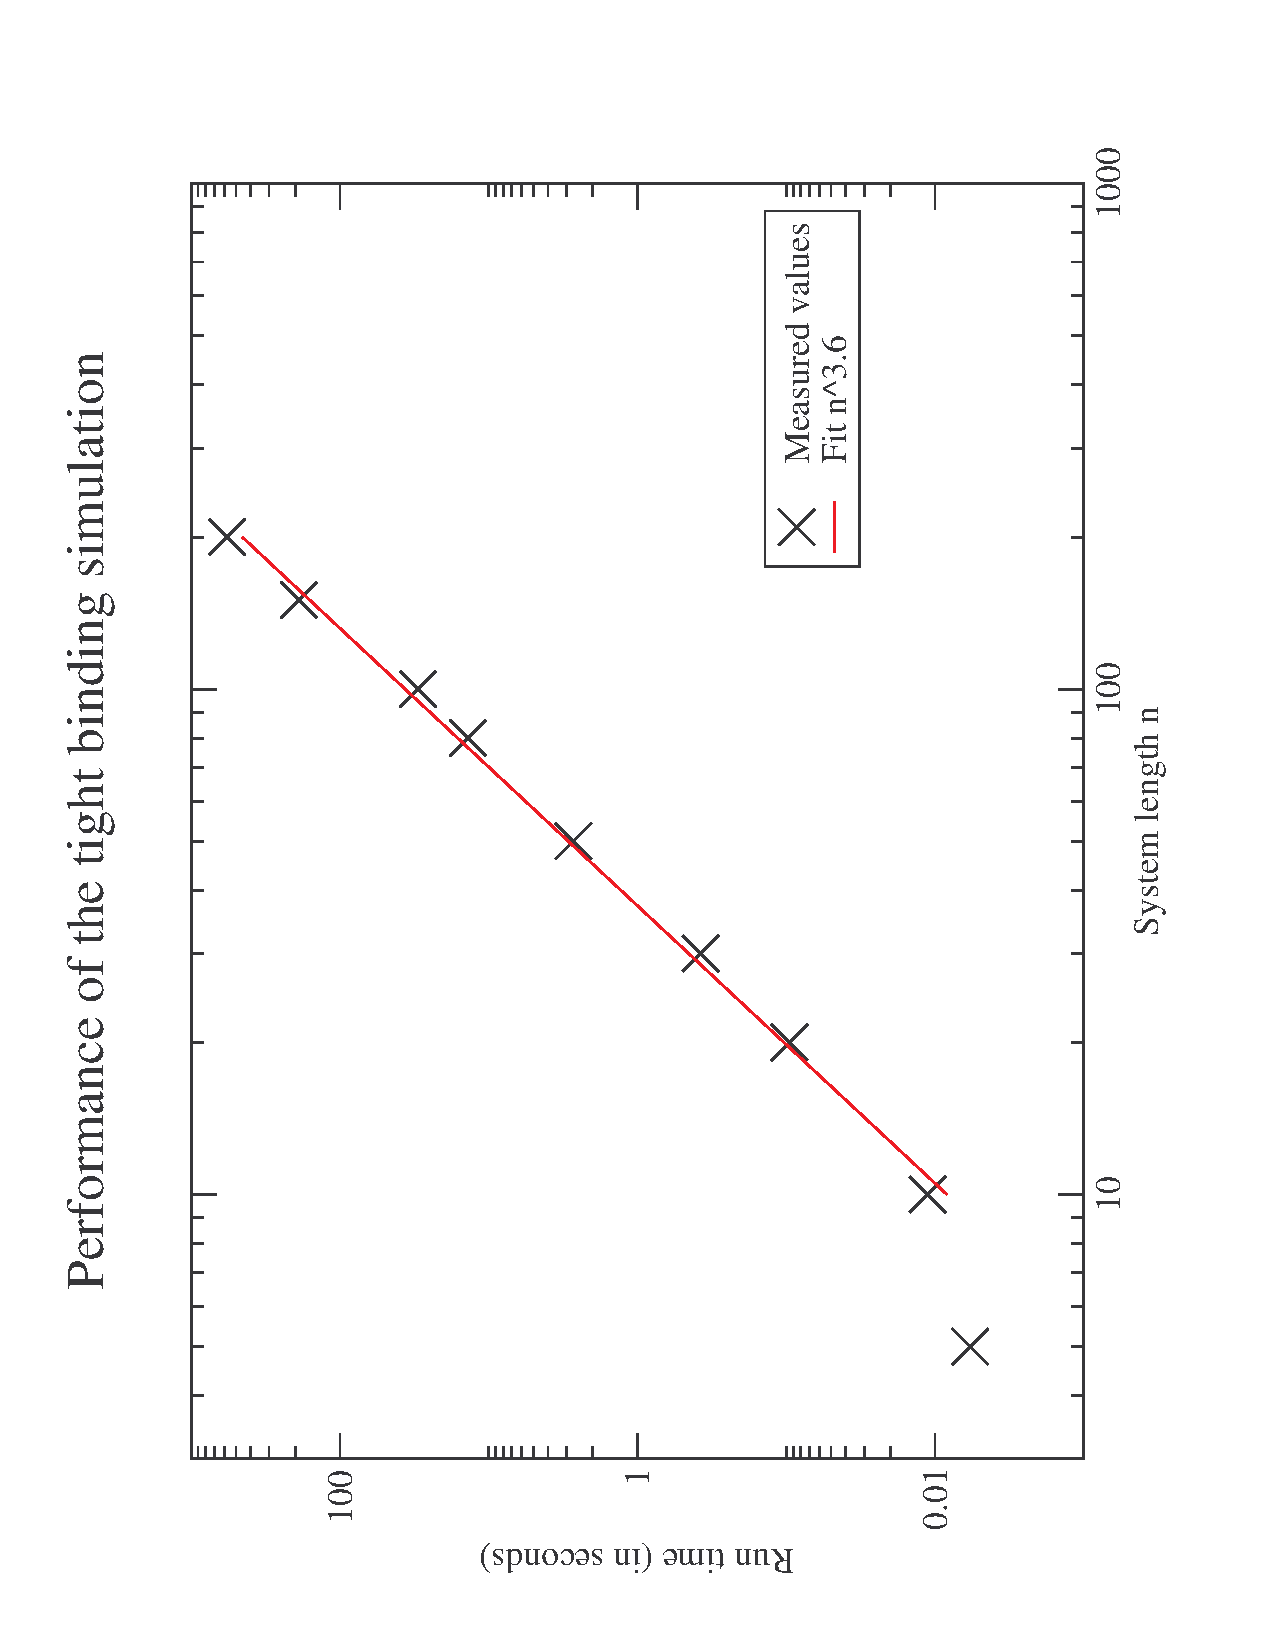
\includegraphics[angle=270,width=0.7\textwidth]{scaling.pdf}
    \end{center}
    \caption{Scaling of run time with system size for the tight binding
        simulation, implemented with sparse matrices and the SuperLU sparse
        direct solver. The data was recorded for square samples including
        Rashba spin-orbit coupling and 4 leads of the same width as the
        sample, on a 2.9GHz AMD64 computer with SSE2 and 8GB RAM.
        The run time approximately scales as $t(n) = 2
        n^{3.64}\mu s$}
        \label{fig:scaling}
\end{figure}

We chose a middle ground: the "naive" approach, but implemented with sparse
matrices and an efficient sparse direct solver \cite{superlu99} for
computing the Green's functions.

The run time thus depends largely on the number of non-zeros in the $H$ and
$\Sigma_p$ and thus on the nature of the interaction. For nearest neighbor
hopping and Rashba spin-orbit coupling, we observed a run time scaling of
$O(n^{3.64})$ (See Fig. \ref{fig:scaling}).

\section{Numerical Stability}

The numerical
calculation uses floating point numbers with limited machine precision,
therefore numerical errors are inevitable.

The transmission matrix for a sample, which is connected to multiple uniform
leads (with same number of modes per lead), has to fulfill the sum rules

\begin{align}
    \sum_p T_{pq} = \sum_q T_{pq} = M
    \label{eq:sumrule}
\end{align}

where $M$ is the number of modes (and thusly and integer). We can calculate
this left hand side of this equation from the numerical simulation, round it
to the nearest integer and thus estimate the numerical error in $T_{pq}$.

Since generally matrix inversion is numerically worse conditioned than solving
a linear equation system \cite{matrixinversion}, we do not actually compute
$G^A$ and $G^R$, but rather the products $G^A\Sigma_p$ and $G^R\Sigma_q$,
which can be written as solutions of linear equation systems.

\begin{align}
    X_p &= \Sigma_p G^R\\
    X_p^\dagger &= (G^R)^\dagger \Sigma_p^\dagger = G^A \sigma_p^\dagger\\
    \Rightarrow\quad (G^A)^-1 X_p^\dagger &= \Sigma_p^\dagger
    \label{eq:lin_gls}
\end{align}

Eq. \ref{eq:lin_gls} is the form with which linear sparse solvers typically
work. They usually calculate a LU decomposition (they write
$(G^A)^-1 = L \cdot U$, where $L$ is a lower triangular matrix and $U$ an
upper triangular matrix), and directly solve the equation by elimination.
Complex conjugation and transposition of $X_p^\dagger$ finally gives us the
matrix which we need evaluating the Fischer-Lee relation.

\begin{figure}
    \begin{center}
    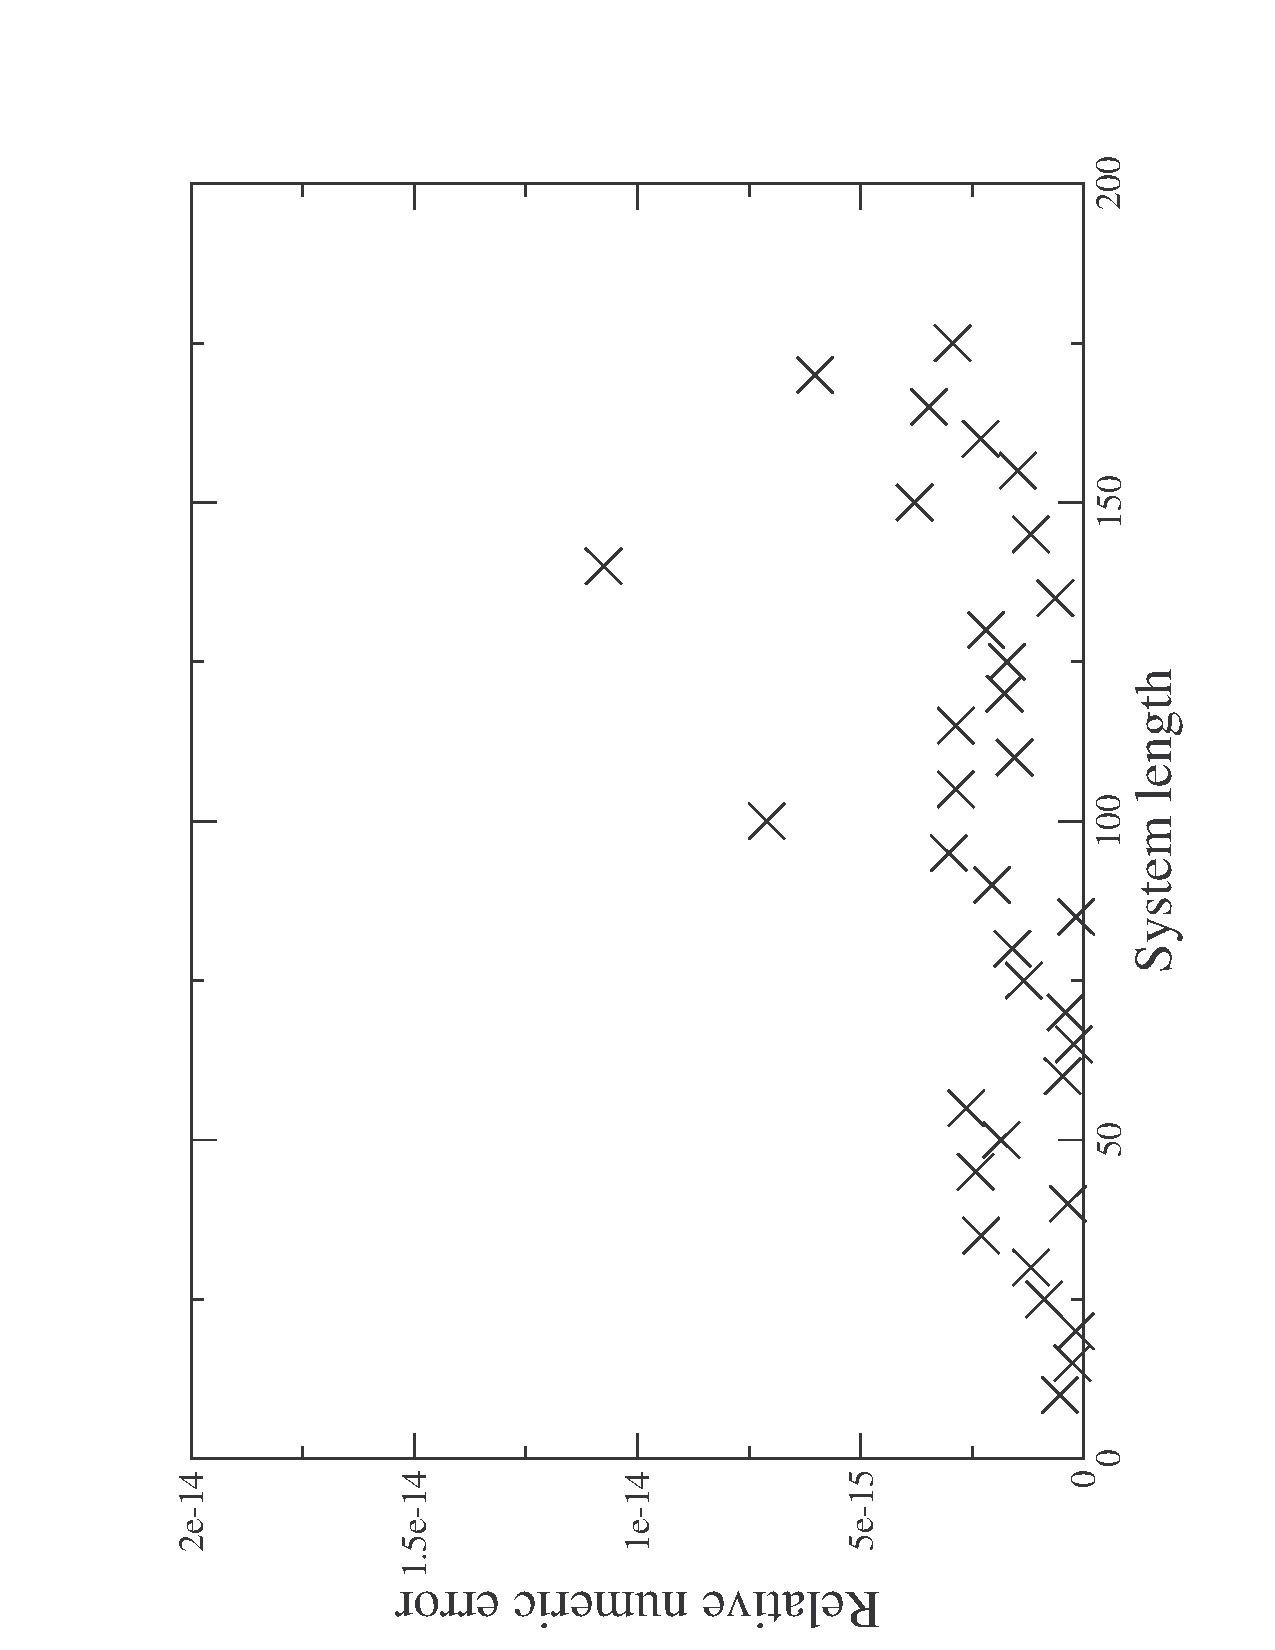
\includegraphics[angle=270,width=0.8\textwidth]{numeric-errors.pdf}
    \end{center}
    \caption{Numerical errors in $T_{pq}$ as a function of system size.}
    \label{fig:numeric-errors}
\end{figure}

Fig. \ref{fig:numeric-errors} shows the estimate of the numerical errors, and
that they are well below $10^{-13}$ for the investigated systems and
thusly are no source for worries.

\section{Quality Checks}

Programming is constantly prone to subtle errors, so measures had to 
be taken to ensure that no errors slipped in that might lead to wrong
output.

The program we discussed herein is basically a function that constructs a
Hamilton operator from the Rashba coupling strength, magnetic
field and other parameters, and then calculates the transmission
matrix $T_{pq}$ from that Hamilton operator.

The very first sanity check is that $H$ is indeed a hermitian
operator. This check, of course, only catches stupid programming
mistakes.

A more elaborate check is that $T_{pq}$ obeys the same symmetries as
the Hamiltonian. Since it can be written as
  
\begin{equation}
H = \frac{\vec{p}^2}{2 m^*} + \vec \sigma \cdot (\vec e_z \times \vec p)  
    + \vec \sigma \cdot \vec B
\end{equation}

it is easy to see that $H(\vec p, \vec \sigma, \vec B) = H(-\vec p,
-\vec \sigma, -\vec B)$, so the transmission matrix must follow the
same symmetries.

We checked these symmetries and the sum rule (eq. \ref{eq:sumrule}) regularly
to ensure that no simple errors slipped in.

\section{Convergence}
\begin{figure}
    \begin{center}
        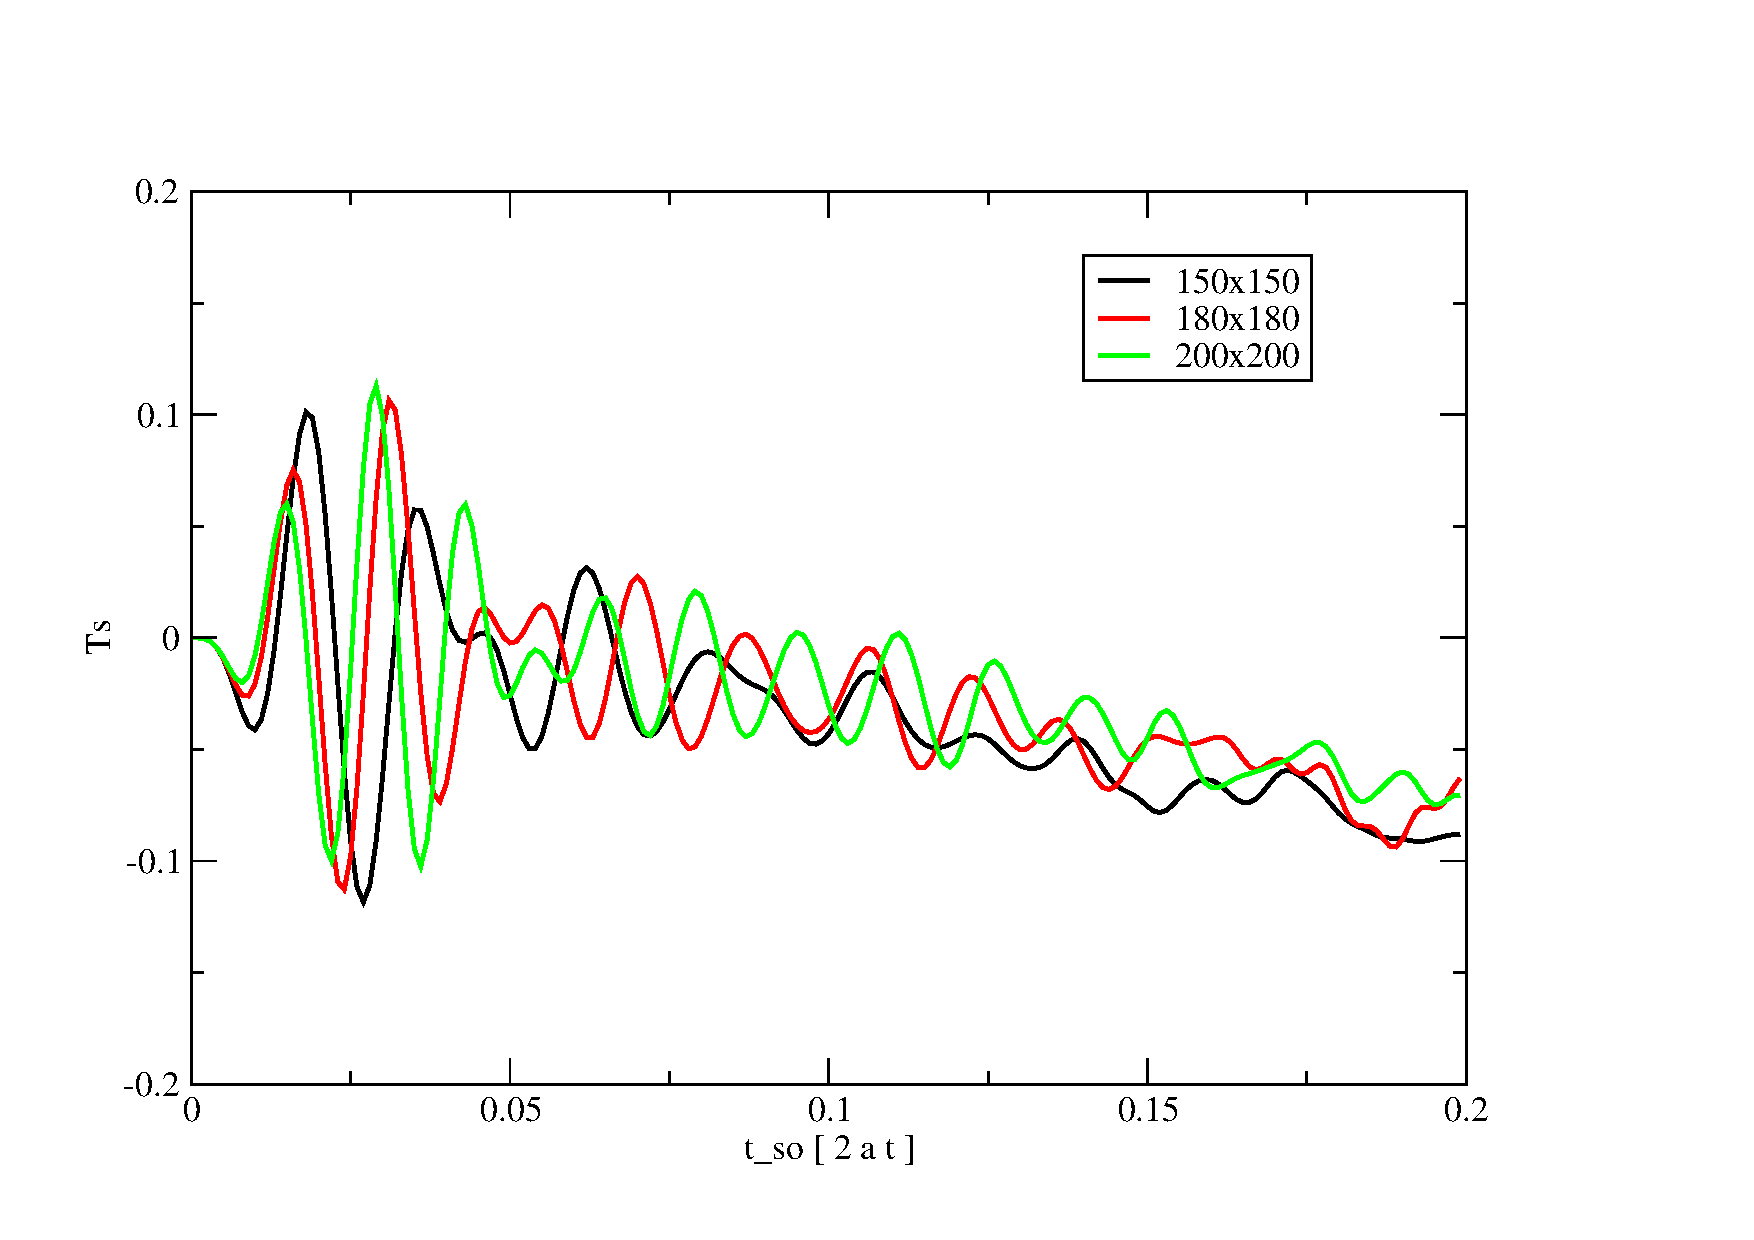
\includegraphics[width=0.8\textwidth]{convergence.pdf}
    \end{center}
    \caption{$T_S = T_{2\uparrow,1\uparrow}-T_{2\downarrow,1\downarrow}$ as a
        function of spin-orbit coupling strength for the setup described in
        section \ref{sec:numeric-setup} with different number of lattice
        sites.}
    \label{fig:convergence}
\end{figure}

The tight binding model is only exactly valid in the limit $ a \mapsto 0$,
i.e. vanishingly small lattice constant. Since the simulation requires a finite
$a$, we have to ensure that the $a$ is actually small enough to not make much
of a difference. This can be done by choosing a smaller $a$ for comparison.

Figure \ref{fig:convergence} shows this for a sample of $100~nm \times 100~nm$.
The results for the resolutions $150 \times 150$, $180 \times 180$ and $200
\times 200$ looks quite similar, but not quite identical. This is because, for
the larger resolution, more modes propagate. Still the qualitative behavior is
sufficiently similar to warrant the use of a $150 \times 150$ grid in the
following simulations.

\section{Setup}
\label{sec:numeric-setup}

\begin{figure}
    \begin{center}
        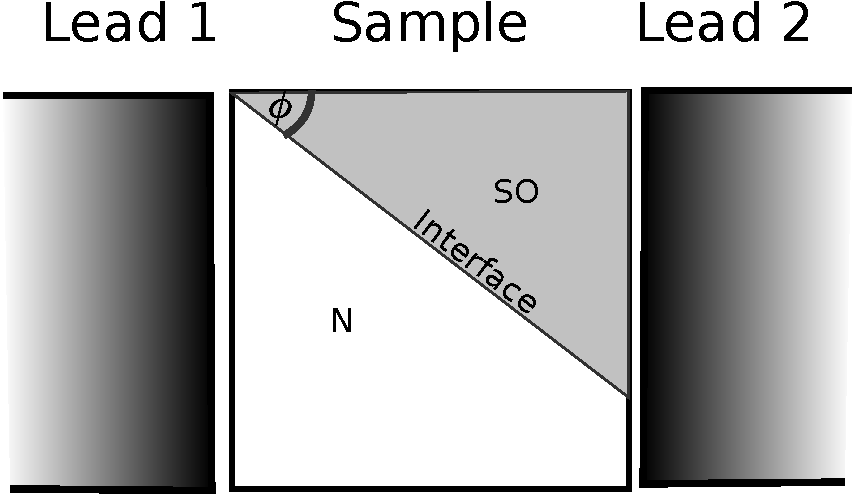
\includegraphics[width=0.5\textwidth]{sample-lead-interface.pdf}%
        \hspace{0.1\textwidth}%
        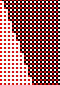
\includegraphics[width=0.2\textwidth]{hopping.png}
    \end{center}
    \caption{\textbf{Left:} The sample is connected to one lead for each spin
        on the left and on the right.
        \textbf{Right:}
        Detail from an interface between normal and spin-orbit coupling regime modeled
        in the tight binding model, at angle $\phi = 70\,^{\circ}$.
        Red dots show lattice sites, black dots
        show non-zero hopping elements with spin flips.}
    \label{fig:interface-setup}
\end{figure}

For the following simulations, we used a square sample, typically of $150
\times 150$ lattice sites, with two leads attached both on the left and on the
right, one for spin up, one for spin down.

\section{Interfaces at Arbitrary Angles}

To simulate an interface of an arbitrary angle $\phi$, we calculate the Rashba
hopping elements separately for each lattice site and install them for
hopping to the right and upper neighbor each. Fig. \ref{fig:interface-setup}
shows how such an interface looks.

\begin{figure}
    \begin{center}
        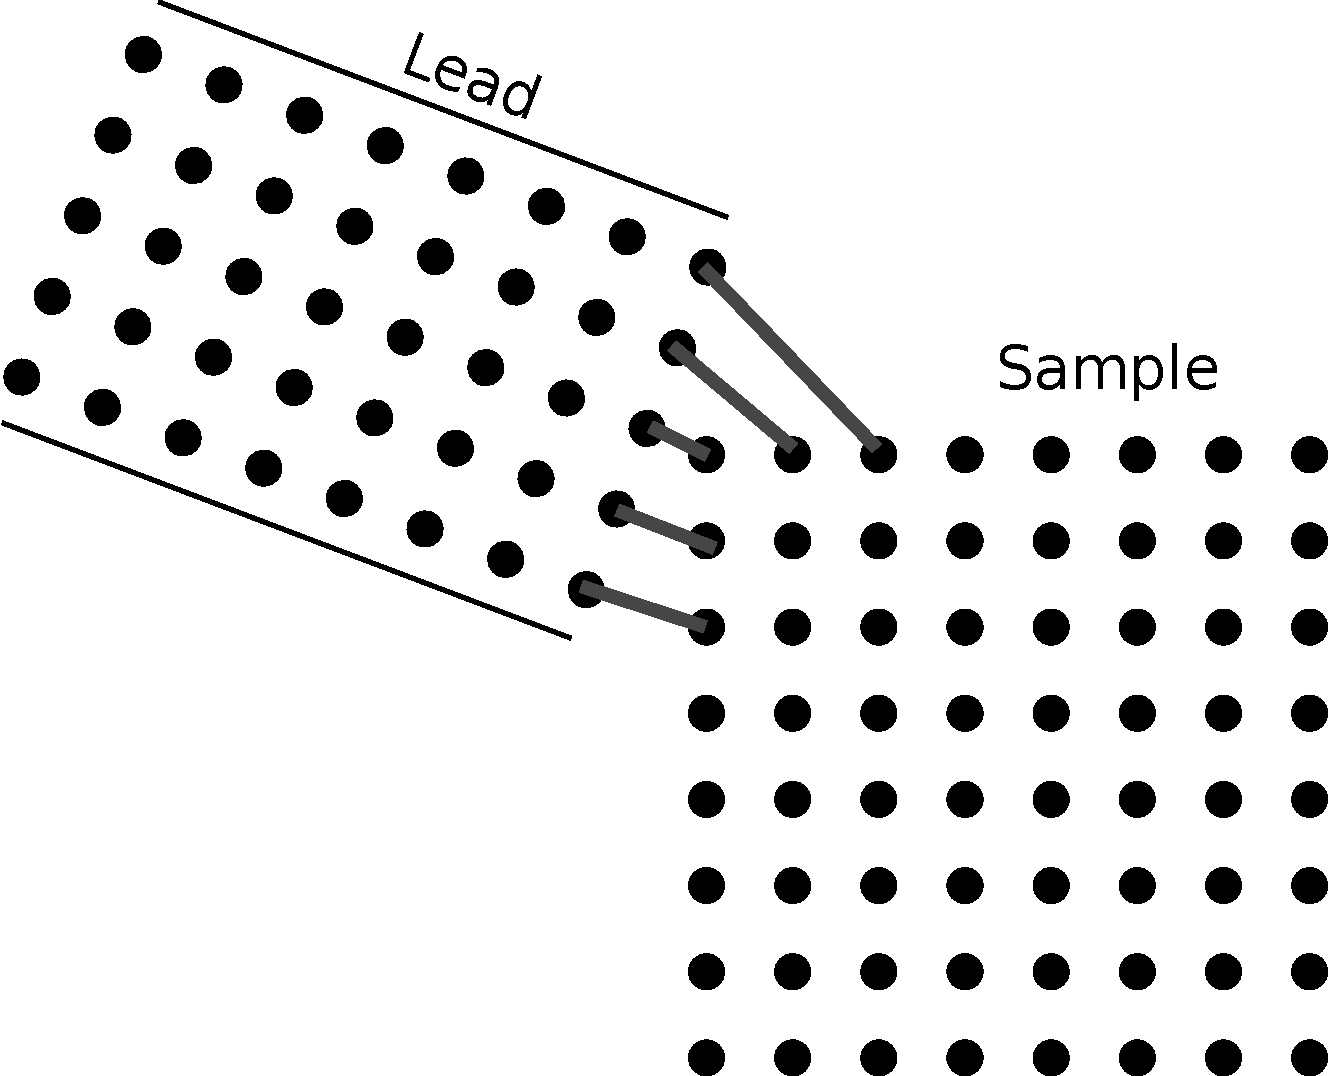
\includegraphics[width=0.4\textwidth]{lead-tilted-1.pdf}
        \hspace{0.1\textwidth}
        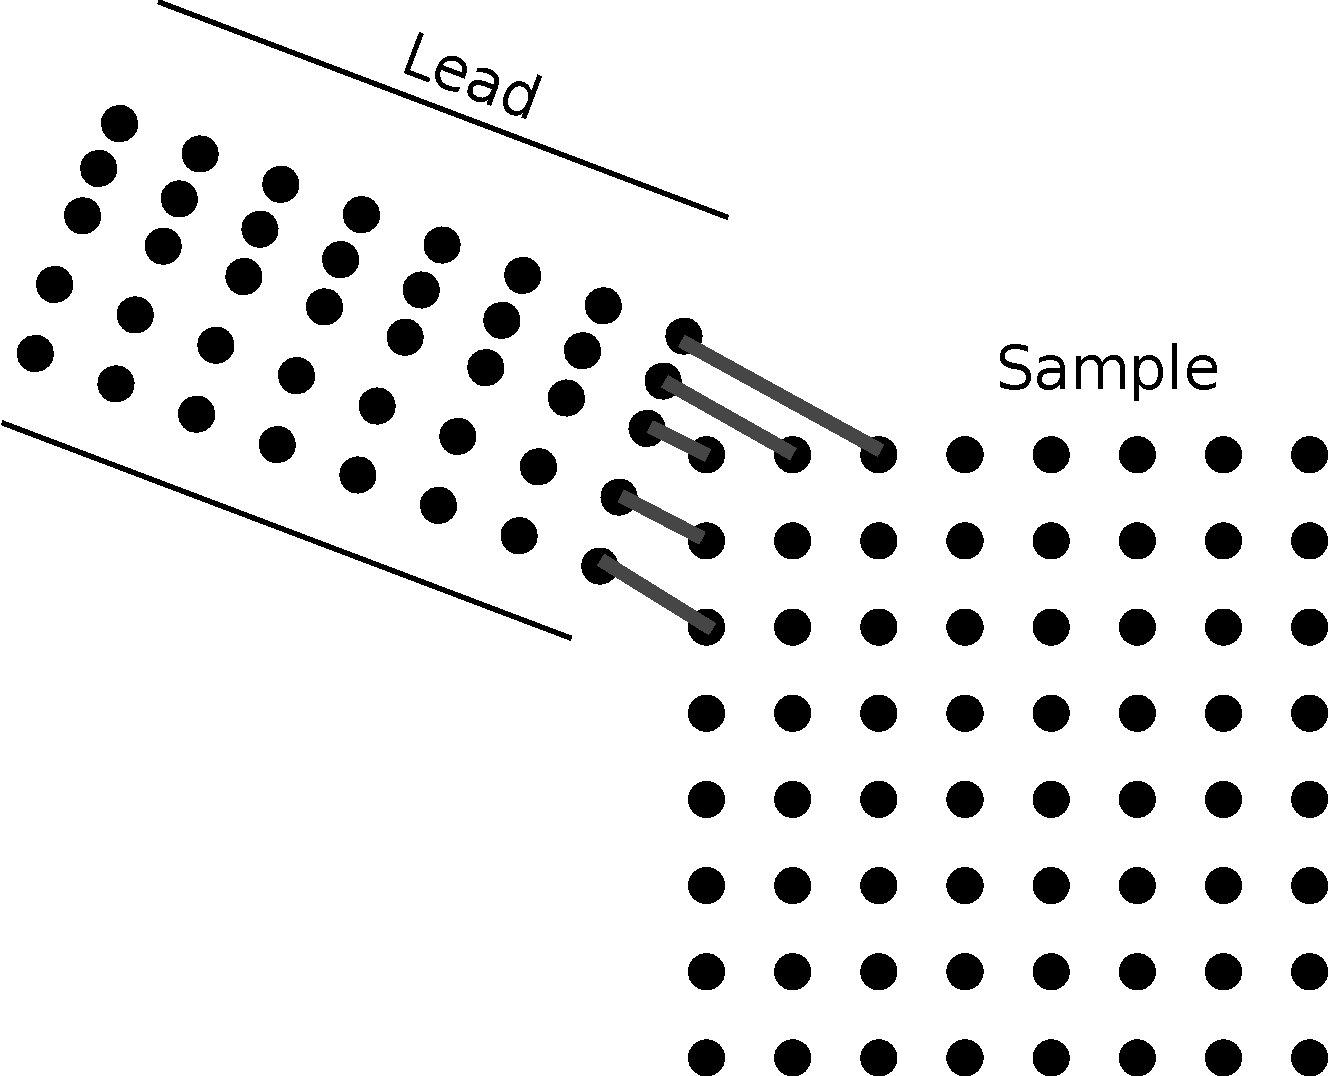
\includegraphics[width=0.4\textwidth]{lead-tilted-2.pdf}
    \end{center}
    \caption{Two ways to attach a tilted lead. \textbf{Left:} Equal lattice
        spacing in lead and sample. \textbf{Right:} Parallel projection from
        the sample into the lead leads to uneven lattice spacing in the lead.}
    \label{fig:tilted-leads}
\end{figure}

To obtain a smoother interface, we also experimented with using a vertical
interface, and injecting the electron beam with a defined angle through a tilted lead.

There are two possible
ways to do this (as illustrated by figure \ref{fig:tilted-leads}):
either one can assume the same lattice spacing in lead and sample and assume
coupling even though the geometry does not match, or one can project the sites
from the edge of the sample parallel into the lead and then get a non-regular
lattice spacing in the lead.

The former turned out not to work the way we wanted it to: instead of one
electron beam propagating in the same direction as the lead, there were two
beams, one parallel to each side of the edge of the sample. The latter is
physically hard to interpret and also much effort to implemented, so we set
that idea aside.

\section{Interface Between Normal and Spin-Orbit Coupling Region}

\begin{figure}
    \begin{center}
    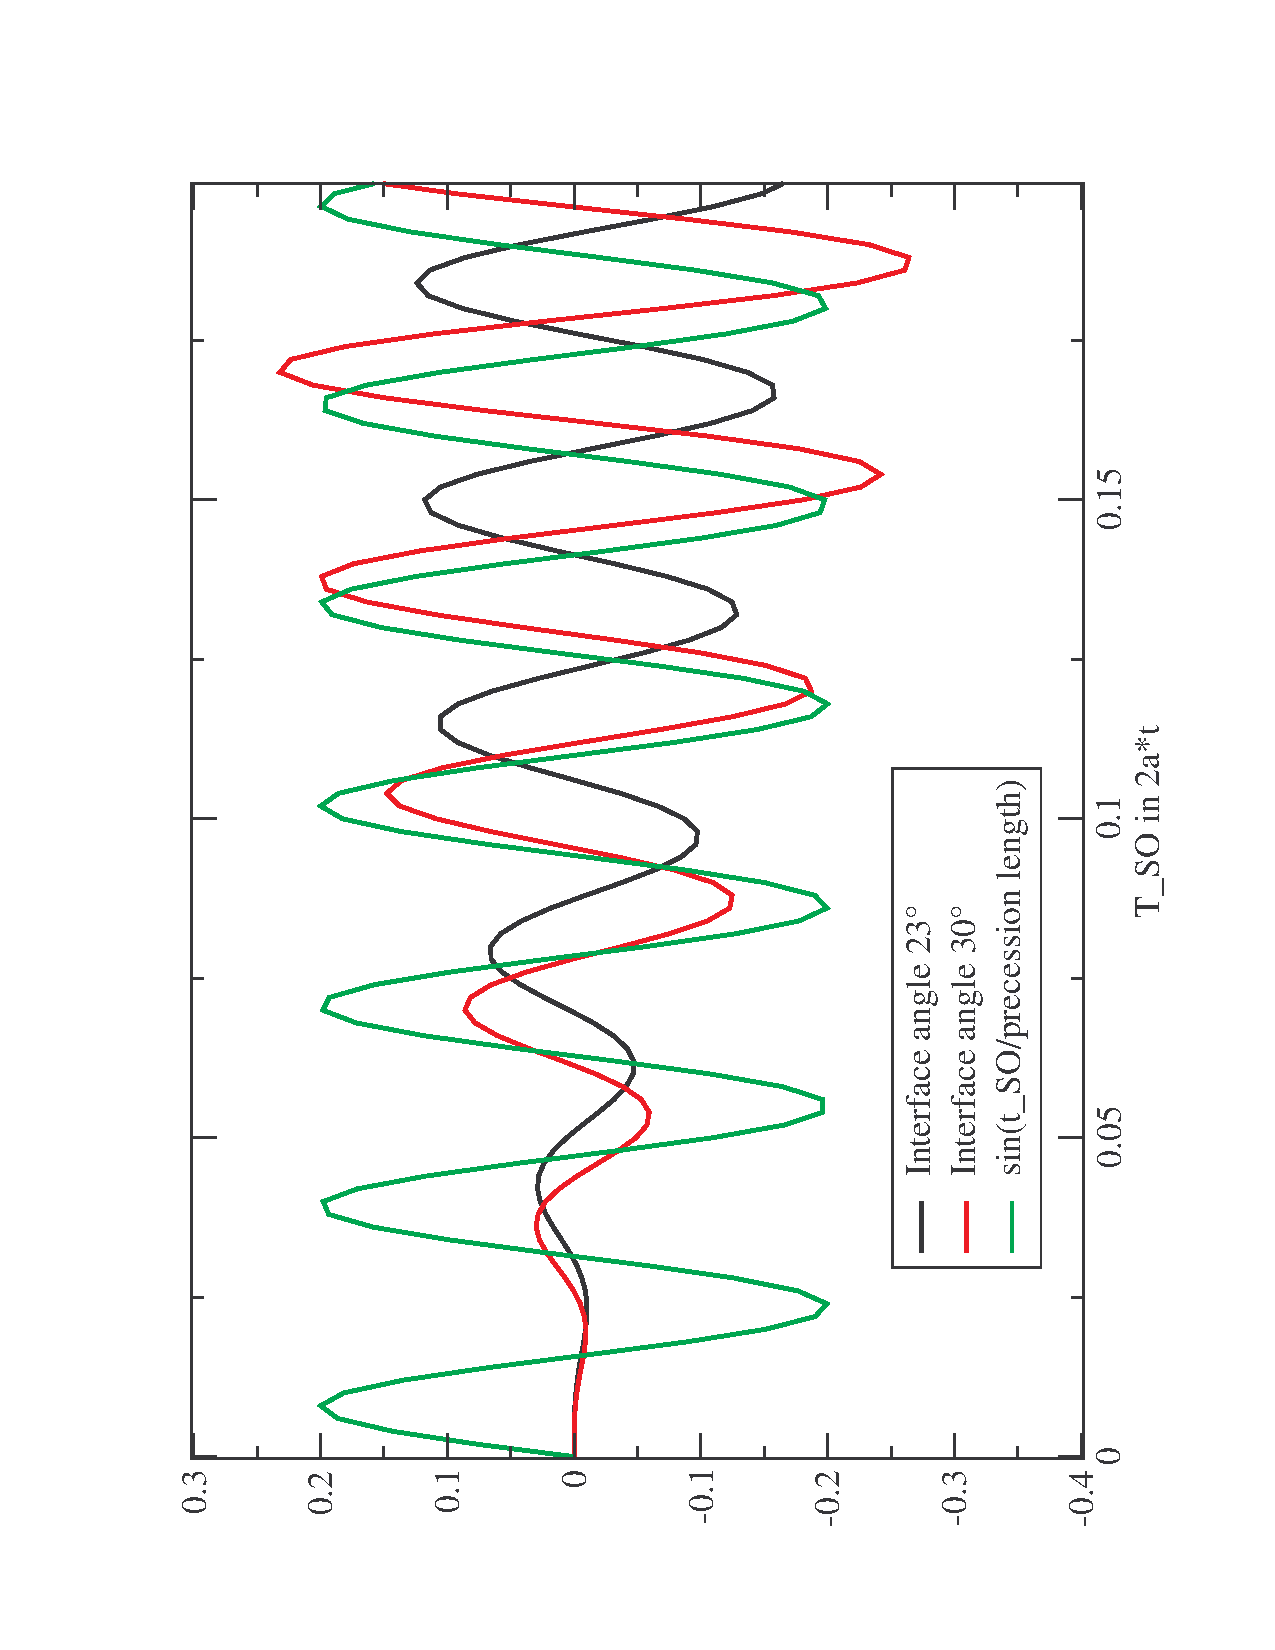
\includegraphics[angle=270,width=0.7\textwidth]{interface-precession.pdf}
    \end{center}
    \caption{$T_S = T_{2\uparrow,1\uparrow}-T_{2\downarrow,1\downarrow}$ as a
        function of spin orbit coupling strength. The interface causes a
        separation of spins which oscillates and is dependent on the angle of
        the interface.}
    \label{fig:interface-precession}
\end{figure}

When plotting $T_S = T_{2\uparrow,1\uparrow}-T_{2\downarrow,1\downarrow}$ as a
function of spin orbit coupling strength, one sees that the signal oscillates
(see figure \ref{fig:interface-precession}).
This is caused by the well-known % TODO: cite
spin precession: in a medium with spin-orbit coupling, $\sigma_z$ is not a good
quantum number anymore, and the spin precesses. % around what?

So if an electron is injected with spin up,and is measured after the
precession length $\lso = \frac{t}{\tso}\pi a$, it is again found to have
spin up, but, after $\frac12 \lso$ or $\frac32 \lso$, the spin points
downwards. 

Since  $\lso$ is a function of $\tso$, the precession can also be
observed when $\tso$ is varied (and not the width of the sample).
If $n$ is an integer and $W$ the width of our sample, we should see the
same signal for $W = n \cdot \lso(n)$ and $W = (n+1) \lso(n+1)$. So
$\tso(n) = n\frac{\pi t}{W}$ and $\Delta \tso = \frac{\pi t}{W}$.  The green
curve in figure \ref{fig:interface-precession} shows the curve
$\sin{\frac{2 \pi \tso}{\Delta \tso}}$ and thus the expected spin precession.

Only a part of the sample has non-zero spin-orbit coupling strength, so $T_S$
actually precesses with a slightly longer period than $\Delta \tso$.

\subsection{Comparison to Analytical Results}

The chiral spin bases as introduced in chapter \ref{sec:analytical} are very
natural for the analytical calculation, because the
base vectors are also eigenstates to the Hamiltonian.

One might think that the easiest way to compare analytical and numerical
results is to simply use the chiral bases in the leads, but that is a
misconception. The chiral spin bases depend on the real space direction
of the waves, and, in the SO regime thus not known a priori --
rather it is an intermediate
result of the numerical calculation\footnote{but one we are not really
interested in, and, by using the Fisher-Lee relation, we shortcut the path and
never explicitly calculate it.}.

So since one can not match the bases between SO region and right lead in the
simulation, one has
to project onto the bases of the leads. We use the $\uparrow,\downarrow$ bases
in the leads, because they are easier to handle.

\begin{figure}
    \begin{center}
    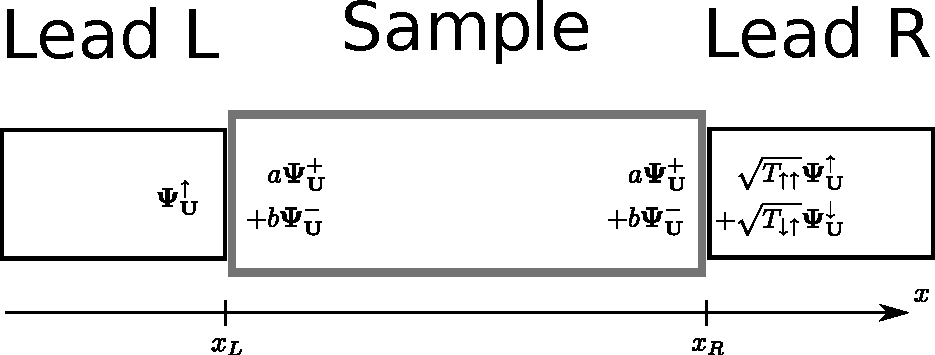
\includegraphics[width=0.8\textwidth]{adapting-pic.pdf}
    \end{center}
    \caption{Injecting one spin-up charge carrier into the system}
\end{figure}

% Since there is no dissipation in our model, and we assume that the mere
% process of injecting an electron doesn't change its spin, we can project
% the $|\uparrow>$ and $|\downarrow>$ states separately onto the wave
% function in the sample:

Since we assume that our leads are perfect semi-infinite wires, we can assume
that the wave functions are plain waves

\begin{align*}
    \mathbf{\Psi^\uparrow}   &=  e^{i p_x x} e^{i p_z z} |\uparrow> \\
    \mathbf{\Psi^\downarrow} &=  e^{i p_x x} e^{i p_z z} |\downarrow> \\
\end{align*}

and that the part of wave function in the sample which travels from left to
right is a smooth continuation of the wave function in the lead:

\begin{align}
    \mathbf{\Psi^\uparrow}(x=x_1) &=
        a\cdot e^{i p_x x_1}e^{i p_z z} \chi_N^+
        + b\cdot e^{i p_x x_1}e^{i p_z z} \chi_N^-\nonumber\\
    \mathbf{\Psi^\downarrow}(x=x_1) &=
        c\cdot e^{i p_x x_1}e^{i p_z z} \chi_N^+
        + d\cdot e^{i p_x x_1}e^{i p_z z} \chi_N^-
        \label{eq:a-n-left}
\end{align}

where $x_1$ is the location where the left lead is connected to the sample, the
interface is at $x = 0$ and the right lead is connected at $x = x_2$.
Each of these equations has two components, which allows us to determine
the coefficients $a, b, c$ and $d$ unambiguously.


We can then look at the connection to the right lead and obtain the 
elements of the transmission matrix in the $\uparrow, \downarrow$ bases:

\begin{align}
    T_{2\uparrow,1\uparrow} = \left| \left( 
        a \mathbf{\Psi^+}(x=x_2) + b  \mathbf{\Psi^-}(x=x_2)
    \right)^\dagger \cdot \mathbf{\Psi}^\uparrow(x=x_2) \right|^2\nonumber\\
    T_{2\downarrow,1\uparrow} = \left| \left( 
        a \mathbf{\Psi^+}(x=x_2) + b  \mathbf{\Psi^-}(x=x_2)
    \right)^\dagger \cdot \mathbf{\Psi}^\downarrow(x=x_2) \right|^2\nonumber\\
    T_{2\uparrow,1\downarrow} = \left| \left( 
        c \mathbf{\Psi^+}(x=x_2) + d  \mathbf{\Psi^-}(x=x_2)
    \right)^\dagger \cdot \mathbf{\Psi}^\uparrow(x=x_2) \right|^2\nonumber\\
    T_{2\downarrow,1\downarrow} = \left| \left( 
        c \mathbf{\Psi^+}(x=x_2) + d  \mathbf{\Psi^-}(x=x_2)
    \right)^\dagger \cdot \mathbf{\Psi}^\downarrow(x=x_2) \right|^2
%    \label{eq:an-right}
\end{align}

where $\mathbf{\Psi^\pm}$ are the wave functions introduced in
\ref{eq:chiral-wafe-function}. Note that these wave functions are not
normalized in the usual sense. Rather on the left of the interface ($x < 0$),
they consist of a part traveling left to right, and a part traveling right to
left. The left-to-right part is normalized the same way as
$\mathbf{\Psi^\uparrow}$
is.

Both the right-to-left part of $\mathbf{\Psi^\pm}(x < 0)$ and the whole of
$\mathbf{\Psi^\pm}(x > 0)$ are not normalized, and in magnitude generally
smaller than 1 which allows us to determine the transmission matrix elements
by looking at the amplitudes.

For comparing the analytical and numeric results, one final step is missing:
$\tso$ and $\ta$ are not the same, but it is easy to get a relation between the
two:

\begin{align}
    \tso &= \frac{\alpha\hbar}{2a}\\
    t    &= \frac{\hbar^2}{2 m a^2}\\
    \frac{\tso}{t} &= \frac{\alpha m a}{\hbar} = \frac{\ta v_F m a}{\hbar} \\
    \Rightarrow \frac{\tso}{t \ta} &= a k_F = a \sqrt{2 \pi n_{2D}}
\end{align}

where $k_F$ is the Fermi wave vector and $n_{2D} \approx 10^{11} cm^{-2}$ is
the density of states in two dimensions.

\begin{figure}
    \begin{center}
        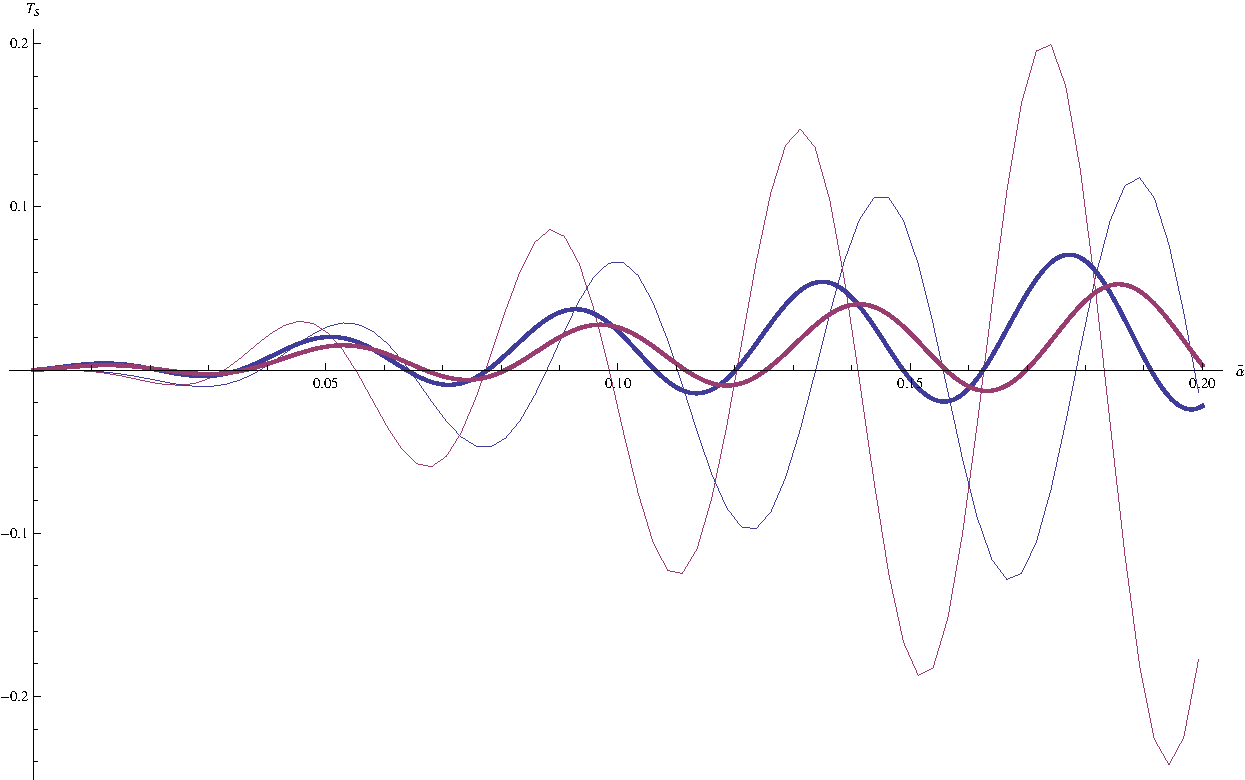
\includegraphics[width=0.8\textwidth]{comparison-over-alpha.pdf}
    \end{center}
    \caption{$T_S = T_{2\uparrow,1\uparrow} - T_{2\downarrow,1\downarrow}$ as
        a function of $\ta$. Bold curves show the results from the analytical
        calculations, thin lines from the numerical calculation.
        \textbf{Blue:} $\phi = 23^\circ$, \textbf{Red:} $\phi = 29^\circ$.
    }
    \label{fig:a-n-matching-alpha}
\end{figure}
\begin{figure}
    \begin{center}
        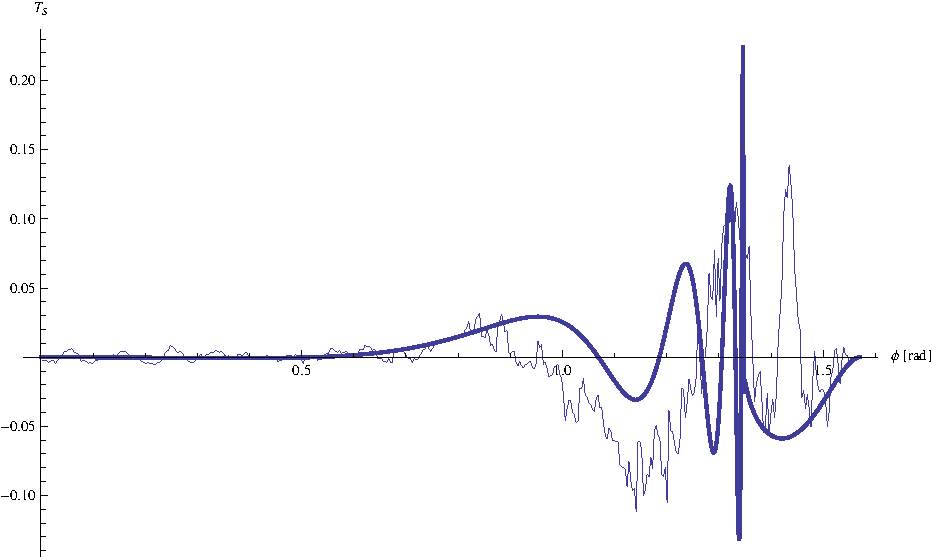
\includegraphics[width=0.8\textwidth]{comparison-over-phi.pdf}
    \end{center}
    \caption{$T_S = T_{2\uparrow,1\uparrow} - T_{2\downarrow,1\downarrow}$ as
        a function of the interface angle $\phi$ (in radians). The bold curve
            show the result from the analytical calculations, the thin line
            from the numerical calculation. $\tso = 0.02$, $E_F = 1.5t$
    }
    \label{fig:a-n-matching-phi}
\end{figure}
\begin{figure}
    \begin{center}
        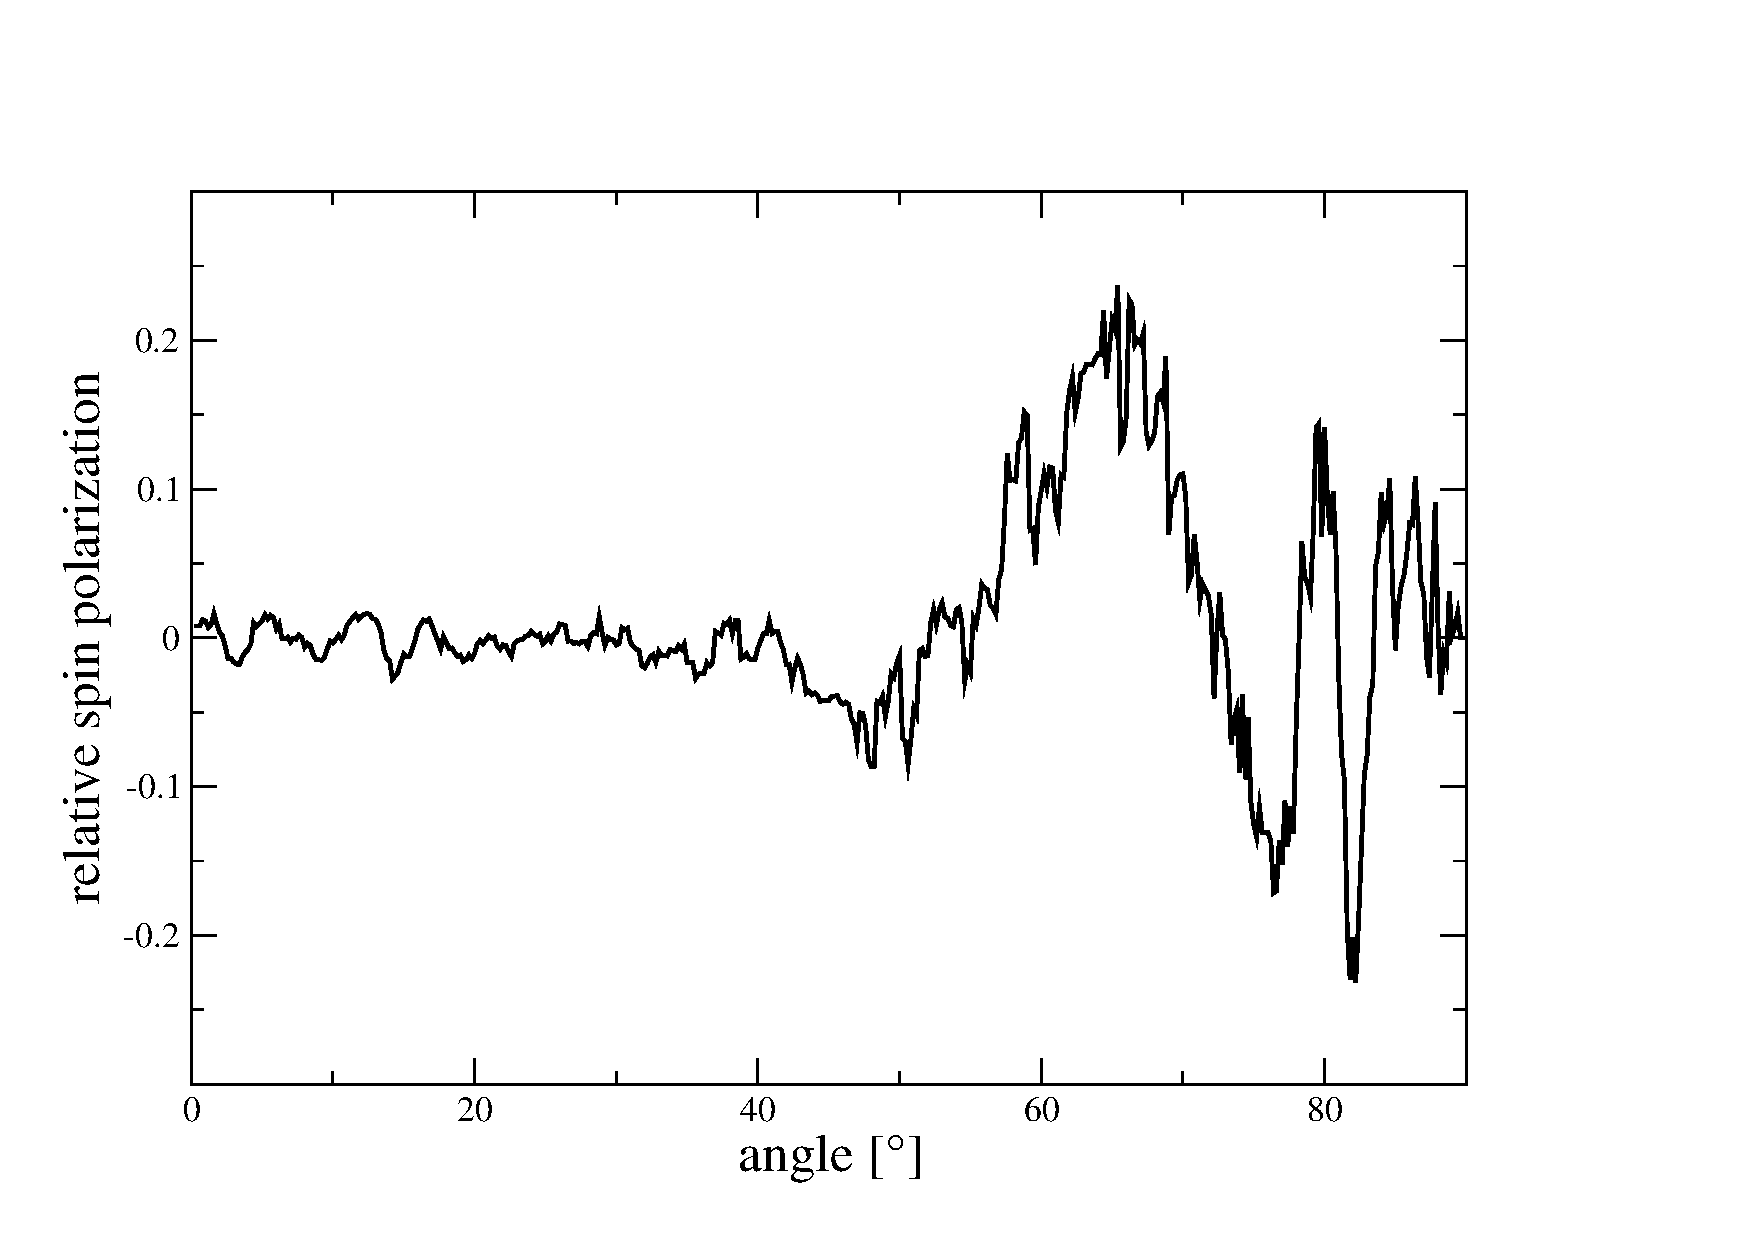
\includegraphics[width=0.8\textwidth]{relative-polarization-n-so.pdf}
    \end{center}
    \caption{$T_S^{rel} = \frac{T_{2\uparrow,1\uparrow} - T_{2\downarrow,1\downarrow}}
        {T_{2\uparrow,1\uparrow} + T_{2\downarrow,1\downarrow}}$ as
        a function of the interface angle $\phi$ (in degrees), and otherwise
        identical parameters as in fig. \ref{fig:a-n-matching-phi}.
        We observe a maximal spin polarization of about $20\%$.
        }
    \label{fig:n-so-rel}
\end{figure}

Figure \ref{fig:a-n-matching-alpha} shows the signal for two different
angles of the interface. For weak spin-orbit coupling, the theory and the
numerical results agree well, for stronger coupling both the oscillation
period and the amplitude start to disagree.

Figure \ref{fig:a-n-matching-phi} shows the effect of the interface angle
$\phi$ as for a fixed spin-orbit coupling strength. The signal from the
numerical simulation is quite noisy, because
a small variation of $\phi$ moves the steps that are used to emulate a smooth
interface.

In order to get one propagating mode in most of the sample, a rather
high Fermi energy was chosen ($E_F = 1.5t$), which means that $k_F$ is
actually quite large. The tight binding simulation only works well for small
wave vectors where the parabolic band can be well approximated with the
cosine form that the tight binding model implies. This explains why there is a
shift between the two curves in figure \ref{fig:a-n-matching-phi}.

For a rather small spin-orbit coupling strength of $\frac{\tso}{2 t a} = 0.02$
we already get a quite respectable relative spin-polarization of $20\%$.

To understand better why we don't get a very clear picture of the critical
angle the numerical results, we look at \ref{eq:a-n-left} and for a moment
ignore the global phases that the $\exp$ functions provide, and obtain a
simplified expression for $a$ and $b$.

\begin{align}
   a &= \frac{1-\sin \phi}{1 + \sin\phi} \nonumber\\
   b &= \sqrt{1-a^2}
\end{align}

Since $t_{-+}$ and $t_{+-}$ are rather small, we also neglect them, as well as
the $exp$ functions in $\mathbf{\Psi^\pm}$, which only contribute phases for
$\phi < \phi_c$. Thus we obtain approximate, 
simplified expression for our matrix elements:

\begin{align}
    T_{2\uparrow,1\uparrow}     &\approx \left|a \chi_{SO}^{+U} t_{++}
            + b \chi_{SO}^{-U} t_{--} \right|^2\\
    T_{2\downarrow,1\downarrow} &\approx \left|c \chi_{SO}^{-D} t_{--}
            + d \chi_{SO}^{+D} t_{--} \right|^2
\end{align}

where the superscript index $U$ means \emph{upper component of}, and $D$ means
\emph{lower component of}.

When $\phi$ is varied in the range of 0 to $\pi/2$, the coefficients $a, b, c,
d$ and the absolute values of the spinor components cover the range of 0 to 1.
The critical phenomena and the variation of $t_{++}$ and $t_{--}$ drown in
eight parameters which oscillate roughly with the same frequency and
magnitude, washing out a clear signature from the chiral waves.

Or speaking more in terms of physical quantities, the interface efficiently
selects waves of $-$ chirality over waves of $+$ chirality (for large angles),
but injecting and measuring the waves in the $\uparrow,\downarrow$ bases
hides a significant part of this effect.

\section{Interface Between Two Spin-Orbit Coupling Regions}

\begin{figure}
    \begin{center}
        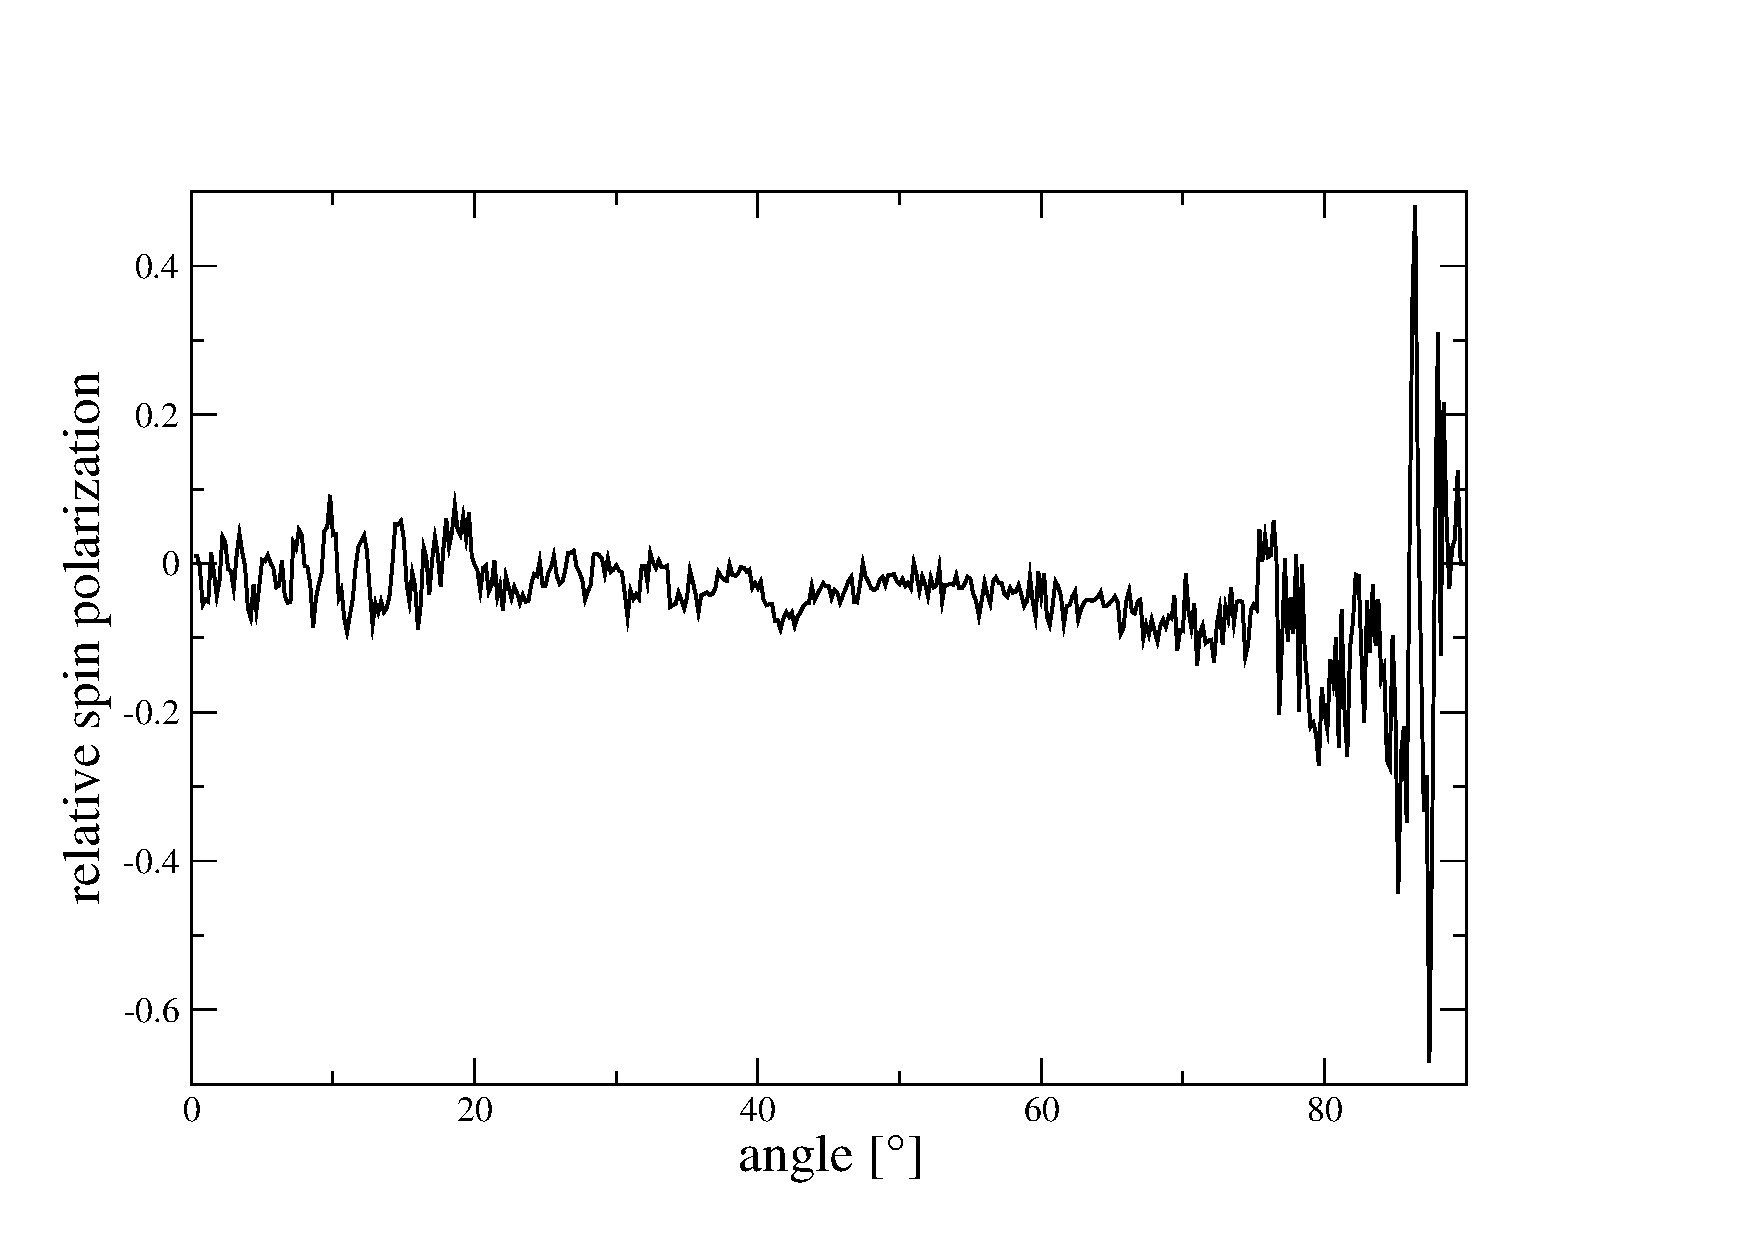
\includegraphics[width=0.8\textwidth]{relative-polarization-so-so.pdf}
    \end{center}
    \caption{$T_S^{rel} = \frac{T_{2\uparrow,1\uparrow} - T_{2\downarrow,1\downarrow}}
        {T_{2\uparrow,1\uparrow} + T_{2\downarrow,1\downarrow}}$ as
        a function of the interface angle $\phi$ (in degrees), for an
        interface of two non-zero spin-orbit coupling regions. $t_{SO,B} =
        \frac{0.1}{2 a t}$, $t_{SO,A} = 0.5 t_{SO,B}$. As in the case of
        a N and SO region, we can observe a spin polarization of about $20\%$,
          with additional peaks going up to about $40\%$.
        ($150 \times 150$ sample of $100~nm \times 100~nm$ at $E_F = 2 t$)
        }
    \label{fig:n-so-rel}
\end{figure}

When a sample contains a 2-dimensional electron gas with Rashba spin-orbit
coupling, it is very hard to create a region without any spin-orbit coupling.
While it is hard to switch it off entirely, it is quite possible to tune the
strength of an individual region by using a gate electrode on top of the
sample to apply an electric field.

Figure \ref{fig:n-so-rel} shows the relative spin polarization as a function
of the interface angle $\phi$, for $\ta_B = 2 \ta_A$. Again a spin
polarization of $20\%$ can be observed, with some few spikes going up as high
as $40\%$ (but with stronger SO interaction on the right-hand side than in the
case of the N-SO interface).

%For $\phi > \phi_c$, the wave $\exp{i p_x^+ x}\exp{i p_z z} t_{++}\chi_{SO}^+$
%does not propagate, because $p_x^+$ is imaginary. That means that the relative
%spin polarization caused by the $\mathbf{\Psi^+}$ wave
%is  the difference of squares of the components of $\chi_{SO}^-$
%(see equation \ref{eq:chi-so-pm} for the explicit form of $\chi_{SO}^-$).

%\begin{align}
%    |T_s^{\textnormal{rel}}| &= \left| \frac{T_{2\uparrow,1\uparrow} -
%        T_{2\downarrow,1\downarrow}}{T_{2\uparrow,1\uparrow}
%            +T_{2\downarrow,1\downarrow}} \right| \nonumber \\
%        &= \frac{\left| |p^+_{SO} - p_{x,SO}^+|^2 -
%    p_z^2\right|}{|p_{SO}^+ - p_{x,SO}^+|^2 + p_z^2} \qquad \textnormal{ for }
%    \phi > \phi_c
%\end{align}
%
%\begin{figure}
%    \begin{center}
%        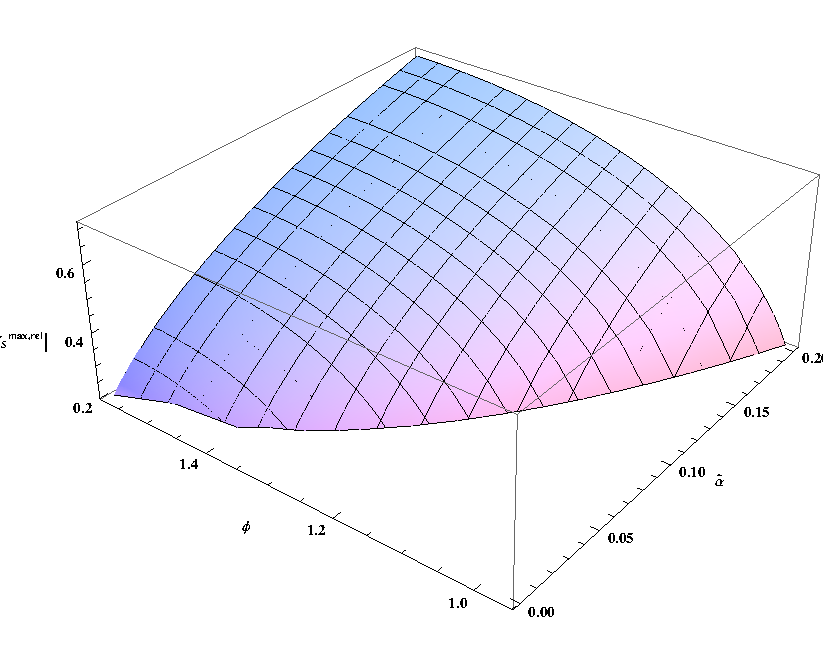
\includegraphics[width=0.8\textwidth]{max-spin-polarization.pdf}
%    \end{center}
%    \caption{Relative spin polarization above the critical angle
%        $\phi_c$ as caused by the incident wave with $+$ chirality}
%\end{figure}

% vim: ts=4 sw=4 expandtab spell spelllang=en_us tw=78
